\documentclass{standalone}
\usepackage{tikz}
\usetikzlibrary{decorations.pathreplacing,decorations.pathmorphing}
\usetikzlibrary{fit,quotes}
\usepackage{yquant, braket}

\begin{document}

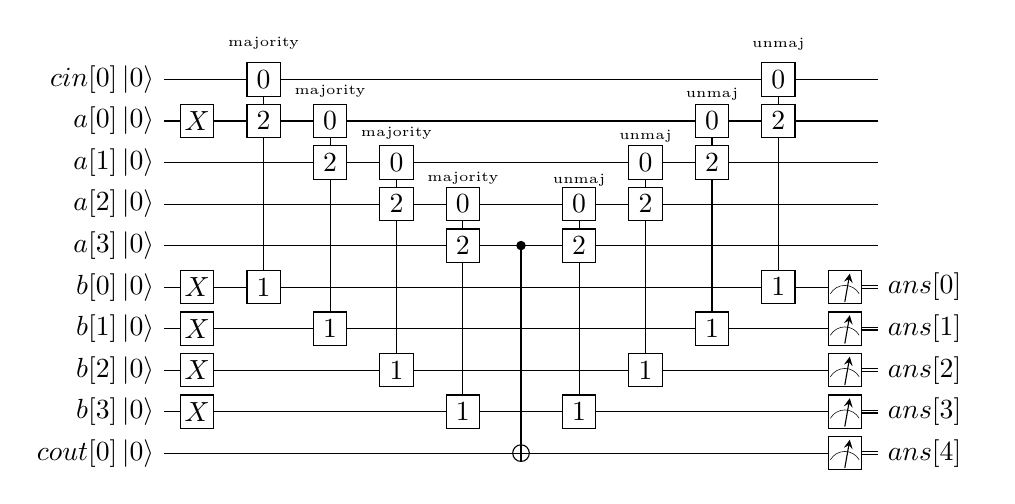
\begin{tikzpicture}[scale=1.000000,x=1pt,y=1pt]
\filldraw[color=white] (0.000000, -7.500000) rectangle (258.000000, 142.500000);
% Drawing wires
% Line 1: cin0 W cin[0]\ket{0}
\draw[color=black] (0.000000,135.000000) -- (258.000000,135.000000);
\draw[color=black] (0.000000,135.000000) node[left] {$cin[0]\ket{0}$};
% Line 2: a0 W a[0]\ket{0}
\draw[color=black] (0.000000,120.000000) -- (258.000000,120.000000);
\draw[color=black] (0.000000,120.000000) node[left] {$a[0]\ket{0}$};
% Line 3: a1 W a[1]\ket{0}
\draw[color=black] (0.000000,105.000000) -- (258.000000,105.000000);
\draw[color=black] (0.000000,105.000000) node[left] {$a[1]\ket{0}$};
% Line 4: a2 W a[2]\ket{0}
\draw[color=black] (0.000000,90.000000) -- (258.000000,90.000000);
\draw[color=black] (0.000000,90.000000) node[left] {$a[2]\ket{0}$};
% Line 5: a3 W a[3]\ket{0}
\draw[color=black] (0.000000,75.000000) -- (258.000000,75.000000);
\draw[color=black] (0.000000,75.000000) node[left] {$a[3]\ket{0}$};
% Line 6: b0 W b[0]\ket{0} ans[0]
\draw[color=black] (0.000000,60.000000) -- (246.000000,60.000000);
\draw[color=black] (246.000000,59.500000) -- (258.000000,59.500000);
\draw[color=black] (246.000000,60.500000) -- (258.000000,60.500000);
\draw[color=black] (0.000000,60.000000) node[left] {$b[0]\ket{0}$};
% Line 7: b1 W b[1]\ket{0} ans[1]
\draw[color=black] (0.000000,45.000000) -- (246.000000,45.000000);
\draw[color=black] (246.000000,44.500000) -- (258.000000,44.500000);
\draw[color=black] (246.000000,45.500000) -- (258.000000,45.500000);
\draw[color=black] (0.000000,45.000000) node[left] {$b[1]\ket{0}$};
% Line 8: b2 W b[2]\ket{0} ans[2]
\draw[color=black] (0.000000,30.000000) -- (246.000000,30.000000);
\draw[color=black] (246.000000,29.500000) -- (258.000000,29.500000);
\draw[color=black] (246.000000,30.500000) -- (258.000000,30.500000);
\draw[color=black] (0.000000,30.000000) node[left] {$b[2]\ket{0}$};
% Line 9: b3 W b[3]\ket{0} ans[3]
\draw[color=black] (0.000000,15.000000) -- (246.000000,15.000000);
\draw[color=black] (246.000000,14.500000) -- (258.000000,14.500000);
\draw[color=black] (246.000000,15.500000) -- (258.000000,15.500000);
\draw[color=black] (0.000000,15.000000) node[left] {$b[3]\ket{0}$};
% Line 10: cout0 W cout[0]\ket{0} ans[4]
\draw[color=black] (0.000000,0.000000) -- (246.000000,0.000000);
\draw[color=black] (246.000000,-0.500000) -- (258.000000,-0.500000);
\draw[color=black] (246.000000,0.500000) -- (258.000000,0.500000);
\draw[color=black] (0.000000,0.000000) node[left] {$cout[0]\ket{0}$};
% Done with wires; drawing gates
% Line 11: a0 X
\begin{scope}
\draw[fill=white] (12.000000, 120.000000) +(-45.000000:8.485281pt and 8.485281pt) -- +(45.000000:8.485281pt and 8.485281pt) -- +(135.000000:8.485281pt and 8.485281pt) -- +(225.000000:8.485281pt and 8.485281pt) -- cycle;
\clip (12.000000, 120.000000) +(-45.000000:8.485281pt and 8.485281pt) -- +(45.000000:8.485281pt and 8.485281pt) -- +(135.000000:8.485281pt and 8.485281pt) -- +(225.000000:8.485281pt and 8.485281pt) -- cycle;
\draw (12.000000, 120.000000) node {$X$};
\end{scope}
% Line 12: b0 X
\begin{scope}
\draw[fill=white] (12.000000, 60.000000) +(-45.000000:8.485281pt and 8.485281pt) -- +(45.000000:8.485281pt and 8.485281pt) -- +(135.000000:8.485281pt and 8.485281pt) -- +(225.000000:8.485281pt and 8.485281pt) -- cycle;
\clip (12.000000, 60.000000) +(-45.000000:8.485281pt and 8.485281pt) -- +(45.000000:8.485281pt and 8.485281pt) -- +(135.000000:8.485281pt and 8.485281pt) -- +(225.000000:8.485281pt and 8.485281pt) -- cycle;
\draw (12.000000, 60.000000) node {$X$};
\end{scope}
% Line 13: b1 X
\begin{scope}
\draw[fill=white] (12.000000, 45.000000) +(-45.000000:8.485281pt and 8.485281pt) -- +(45.000000:8.485281pt and 8.485281pt) -- +(135.000000:8.485281pt and 8.485281pt) -- +(225.000000:8.485281pt and 8.485281pt) -- cycle;
\clip (12.000000, 45.000000) +(-45.000000:8.485281pt and 8.485281pt) -- +(45.000000:8.485281pt and 8.485281pt) -- +(135.000000:8.485281pt and 8.485281pt) -- +(225.000000:8.485281pt and 8.485281pt) -- cycle;
\draw (12.000000, 45.000000) node {$X$};
\end{scope}
% Line 14: b2 X
\begin{scope}
\draw[fill=white] (12.000000, 30.000000) +(-45.000000:8.485281pt and 8.485281pt) -- +(45.000000:8.485281pt and 8.485281pt) -- +(135.000000:8.485281pt and 8.485281pt) -- +(225.000000:8.485281pt and 8.485281pt) -- cycle;
\clip (12.000000, 30.000000) +(-45.000000:8.485281pt and 8.485281pt) -- +(45.000000:8.485281pt and 8.485281pt) -- +(135.000000:8.485281pt and 8.485281pt) -- +(225.000000:8.485281pt and 8.485281pt) -- cycle;
\draw (12.000000, 30.000000) node {$X$};
\end{scope}
% Line 15: b3 X
\begin{scope}
\draw[fill=white] (12.000000, 15.000000) +(-45.000000:8.485281pt and 8.485281pt) -- +(45.000000:8.485281pt and 8.485281pt) -- +(135.000000:8.485281pt and 8.485281pt) -- +(225.000000:8.485281pt and 8.485281pt) -- cycle;
\clip (12.000000, 15.000000) +(-45.000000:8.485281pt and 8.485281pt) -- +(45.000000:8.485281pt and 8.485281pt) -- +(135.000000:8.485281pt and 8.485281pt) -- +(225.000000:8.485281pt and 8.485281pt) -- cycle;
\draw (12.000000, 15.000000) node {$X$};
\end{scope}
% Line 16: cin0 G $0$ a0 G $2$ b0 G $1$ % majority
\draw (36.000000, 142.500000) node[text width=144pt,above,text centered] {\tiny majority};
\draw (36.000000,135.000000) -- (36.000000,60.000000);
\begin{scope}
\draw[fill=white] (36.000000, 135.000000) +(-45.000000:8.485281pt and 8.485281pt) -- +(45.000000:8.485281pt and 8.485281pt) -- +(135.000000:8.485281pt and 8.485281pt) -- +(225.000000:8.485281pt and 8.485281pt) -- cycle;
\clip (36.000000, 135.000000) +(-45.000000:8.485281pt and 8.485281pt) -- +(45.000000:8.485281pt and 8.485281pt) -- +(135.000000:8.485281pt and 8.485281pt) -- +(225.000000:8.485281pt and 8.485281pt) -- cycle;
\draw (36.000000, 135.000000) node {$0$};
\end{scope}
\begin{scope}
\draw[fill=white] (36.000000, 120.000000) +(-45.000000:8.485281pt and 8.485281pt) -- +(45.000000:8.485281pt and 8.485281pt) -- +(135.000000:8.485281pt and 8.485281pt) -- +(225.000000:8.485281pt and 8.485281pt) -- cycle;
\clip (36.000000, 120.000000) +(-45.000000:8.485281pt and 8.485281pt) -- +(45.000000:8.485281pt and 8.485281pt) -- +(135.000000:8.485281pt and 8.485281pt) -- +(225.000000:8.485281pt and 8.485281pt) -- cycle;
\draw (36.000000, 120.000000) node {$2$};
\end{scope}
\begin{scope}
\draw[fill=white] (36.000000, 60.000000) +(-45.000000:8.485281pt and 8.485281pt) -- +(45.000000:8.485281pt and 8.485281pt) -- +(135.000000:8.485281pt and 8.485281pt) -- +(225.000000:8.485281pt and 8.485281pt) -- cycle;
\clip (36.000000, 60.000000) +(-45.000000:8.485281pt and 8.485281pt) -- +(45.000000:8.485281pt and 8.485281pt) -- +(135.000000:8.485281pt and 8.485281pt) -- +(225.000000:8.485281pt and 8.485281pt) -- cycle;
\draw (36.000000, 60.000000) node {$1$};
\end{scope}
% Line 17: a0 G $0$ a1 G $2$ b1 G $1$ % majority
\draw (60.000000, 125.00000) node[text width=144pt,above,text centered] {\tiny majority};
\draw (60.000000,120.000000) -- (60.000000,45.000000);
\begin{scope}
\draw[fill=white] (60.000000, 120.000000) +(-45.000000:8.485281pt and 8.485281pt) -- +(45.000000:8.485281pt and 8.485281pt) -- +(135.000000:8.485281pt and 8.485281pt) -- +(225.000000:8.485281pt and 8.485281pt) -- cycle;
\clip (60.000000, 120.000000) +(-45.000000:8.485281pt and 8.485281pt) -- +(45.000000:8.485281pt and 8.485281pt) -- +(135.000000:8.485281pt and 8.485281pt) -- +(225.000000:8.485281pt and 8.485281pt) -- cycle;
\draw (60.000000, 120.000000) node {$0$};
\end{scope}
\begin{scope}
\draw[fill=white] (60.000000, 105.000000) +(-45.000000:8.485281pt and 8.485281pt) -- +(45.000000:8.485281pt and 8.485281pt) -- +(135.000000:8.485281pt and 8.485281pt) -- +(225.000000:8.485281pt and 8.485281pt) -- cycle;
\clip (60.000000, 105.000000) +(-45.000000:8.485281pt and 8.485281pt) -- +(45.000000:8.485281pt and 8.485281pt) -- +(135.000000:8.485281pt and 8.485281pt) -- +(225.000000:8.485281pt and 8.485281pt) -- cycle;
\draw (60.000000, 105.000000) node {$2$};
\end{scope}
\begin{scope}
\draw[fill=white] (60.000000, 45.000000) +(-45.000000:8.485281pt and 8.485281pt) -- +(45.000000:8.485281pt and 8.485281pt) -- +(135.000000:8.485281pt and 8.485281pt) -- +(225.000000:8.485281pt and 8.485281pt) -- cycle;
\clip (60.000000, 45.000000) +(-45.000000:8.485281pt and 8.485281pt) -- +(45.000000:8.485281pt and 8.485281pt) -- +(135.000000:8.485281pt and 8.485281pt) -- +(225.000000:8.485281pt and 8.485281pt) -- cycle;
\draw (60.000000, 45.000000) node {$1$};
\end{scope}
% Line 18: a1 G $0$ a2 G $2$ b2 G $1$ % majority
\draw (84.000000, 110.00000) node[text width=144pt,above,text centered] {\tiny majority};
\draw (84.000000,105.000000) -- (84.000000,30.000000);
\begin{scope}
\draw[fill=white] (84.000000, 105.000000) +(-45.000000:8.485281pt and 8.485281pt) -- +(45.000000:8.485281pt and 8.485281pt) -- +(135.000000:8.485281pt and 8.485281pt) -- +(225.000000:8.485281pt and 8.485281pt) -- cycle;
\clip (84.000000, 105.000000) +(-45.000000:8.485281pt and 8.485281pt) -- +(45.000000:8.485281pt and 8.485281pt) -- +(135.000000:8.485281pt and 8.485281pt) -- +(225.000000:8.485281pt and 8.485281pt) -- cycle;
\draw (84.000000, 105.000000) node {$0$};
\end{scope}
\begin{scope}
\draw[fill=white] (84.000000, 90.000000) +(-45.000000:8.485281pt and 8.485281pt) -- +(45.000000:8.485281pt and 8.485281pt) -- +(135.000000:8.485281pt and 8.485281pt) -- +(225.000000:8.485281pt and 8.485281pt) -- cycle;
\clip (84.000000, 90.000000) +(-45.000000:8.485281pt and 8.485281pt) -- +(45.000000:8.485281pt and 8.485281pt) -- +(135.000000:8.485281pt and 8.485281pt) -- +(225.000000:8.485281pt and 8.485281pt) -- cycle;
\draw (84.000000, 90.000000) node {$2$};
\end{scope}
\begin{scope}
\draw[fill=white] (84.000000, 30.000000) +(-45.000000:8.485281pt and 8.485281pt) -- +(45.000000:8.485281pt and 8.485281pt) -- +(135.000000:8.485281pt and 8.485281pt) -- +(225.000000:8.485281pt and 8.485281pt) -- cycle;
\clip (84.000000, 30.000000) +(-45.000000:8.485281pt and 8.485281pt) -- +(45.000000:8.485281pt and 8.485281pt) -- +(135.000000:8.485281pt and 8.485281pt) -- +(225.000000:8.485281pt and 8.485281pt) -- cycle;
\draw (84.000000, 30.000000) node {$1$};
\end{scope}
% Line 19: a2 G $0$ a3 G $2$ b3 G $1$ % majority
\draw (108.000000, 93.500000) node[text width=144pt,above,text centered] {\tiny majority};
\draw (108.000000,90.000000) -- (108.000000,15.000000);
\begin{scope}
\draw[fill=white] (108.000000, 90.000000) +(-45.000000:8.485281pt and 8.485281pt) -- +(45.000000:8.485281pt and 8.485281pt) -- +(135.000000:8.485281pt and 8.485281pt) -- +(225.000000:8.485281pt and 8.485281pt) -- cycle;
\clip (108.000000, 90.000000) +(-45.000000:8.485281pt and 8.485281pt) -- +(45.000000:8.485281pt and 8.485281pt) -- +(135.000000:8.485281pt and 8.485281pt) -- +(225.000000:8.485281pt and 8.485281pt) -- cycle;
\draw (108.000000, 90.000000) node {$0$};
\end{scope}
\begin{scope}
\draw[fill=white] (108.000000, 75.000000) +(-45.000000:8.485281pt and 8.485281pt) -- +(45.000000:8.485281pt and 8.485281pt) -- +(135.000000:8.485281pt and 8.485281pt) -- +(225.000000:8.485281pt and 8.485281pt) -- cycle;
\clip (108.000000, 75.000000) +(-45.000000:8.485281pt and 8.485281pt) -- +(45.000000:8.485281pt and 8.485281pt) -- +(135.000000:8.485281pt and 8.485281pt) -- +(225.000000:8.485281pt and 8.485281pt) -- cycle;
\draw (108.000000, 75.000000) node {$2$};
\end{scope}
\begin{scope}
\draw[fill=white] (108.000000, 15.000000) +(-45.000000:8.485281pt and 8.485281pt) -- +(45.000000:8.485281pt and 8.485281pt) -- +(135.000000:8.485281pt and 8.485281pt) -- +(225.000000:8.485281pt and 8.485281pt) -- cycle;
\clip (108.000000, 15.000000) +(-45.000000:8.485281pt and 8.485281pt) -- +(45.000000:8.485281pt and 8.485281pt) -- +(135.000000:8.485281pt and 8.485281pt) -- +(225.000000:8.485281pt and 8.485281pt) -- cycle;
\draw (108.000000, 15.000000) node {$1$};
\end{scope}
% Line 20: +cout0 a3
\draw (129.000000,75.000000) -- (129.000000,0.000000);
\begin{scope}
\draw[fill=white] (129.000000, 0.000000) circle(3.000000pt);
\clip (129.000000, 0.000000) circle(3.000000pt);
\draw (126.000000, 0.000000) -- (132.000000, 0.000000);
\draw (129.000000, -3.000000) -- (129.000000, 3.000000);
\end{scope}
\filldraw (129.000000, 75.000000) circle(1.500000pt);
% Line 21: a2 G $0$ a3 G $2$ b3 G $1$ % unmaj
\draw (150.000000, 93.00000) node[text width=144pt,above,text centered] {\tiny unmaj};
\draw (150.000000,90.000000) -- (150.000000,15.000000);
\begin{scope}
\draw[fill=white] (150.000000, 90.000000) +(-45.000000:8.485281pt and 8.485281pt) -- +(45.000000:8.485281pt and 8.485281pt) -- +(135.000000:8.485281pt and 8.485281pt) -- +(225.000000:8.485281pt and 8.485281pt) -- cycle;
\clip (150.000000, 90.000000) +(-45.000000:8.485281pt and 8.485281pt) -- +(45.000000:8.485281pt and 8.485281pt) -- +(135.000000:8.485281pt and 8.485281pt) -- +(225.000000:8.485281pt and 8.485281pt) -- cycle;
\draw (150.000000, 90.000000) node {$0$};
\end{scope}
\begin{scope}
\draw[fill=white] (150.000000, 75.000000) +(-45.000000:8.485281pt and 8.485281pt) -- +(45.000000:8.485281pt and 8.485281pt) -- +(135.000000:8.485281pt and 8.485281pt) -- +(225.000000:8.485281pt and 8.485281pt) -- cycle;
\clip (150.000000, 75.000000) +(-45.000000:8.485281pt and 8.485281pt) -- +(45.000000:8.485281pt and 8.485281pt) -- +(135.000000:8.485281pt and 8.485281pt) -- +(225.000000:8.485281pt and 8.485281pt) -- cycle;
\draw (150.000000, 75.000000) node {$2$};
\end{scope}
\begin{scope}
\draw[fill=white] (150.000000, 15.000000) +(-45.000000:8.485281pt and 8.485281pt) -- +(45.000000:8.485281pt and 8.485281pt) -- +(135.000000:8.485281pt and 8.485281pt) -- +(225.000000:8.485281pt and 8.485281pt) -- cycle;
\clip (150.000000, 15.000000) +(-45.000000:8.485281pt and 8.485281pt) -- +(45.000000:8.485281pt and 8.485281pt) -- +(135.000000:8.485281pt and 8.485281pt) -- +(225.000000:8.485281pt and 8.485281pt) -- cycle;
\draw (150.000000, 15.000000) node {$1$};
\end{scope}
% Line 22: a1 G $0$ a2 G $2$ b2 G $1$ % unmaj
\draw (174.000000, 109.00000) node[text width=144pt,above,text centered] {\tiny unmaj};
\draw (174.000000,105.000000) -- (174.000000,30.000000);
\begin{scope}
\draw[fill=white] (174.000000, 105.000000) +(-45.000000:8.485281pt and 8.485281pt) -- +(45.000000:8.485281pt and 8.485281pt) -- +(135.000000:8.485281pt and 8.485281pt) -- +(225.000000:8.485281pt and 8.485281pt) -- cycle;
\clip (174.000000, 105.000000) +(-45.000000:8.485281pt and 8.485281pt) -- +(45.000000:8.485281pt and 8.485281pt) -- +(135.000000:8.485281pt and 8.485281pt) -- +(225.000000:8.485281pt and 8.485281pt) -- cycle;
\draw (174.000000, 105.000000) node {$0$};
\end{scope}
\begin{scope}
\draw[fill=white] (174.000000, 90.000000) +(-45.000000:8.485281pt and 8.485281pt) -- +(45.000000:8.485281pt and 8.485281pt) -- +(135.000000:8.485281pt and 8.485281pt) -- +(225.000000:8.485281pt and 8.485281pt) -- cycle;
\clip (174.000000, 90.000000) +(-45.000000:8.485281pt and 8.485281pt) -- +(45.000000:8.485281pt and 8.485281pt) -- +(135.000000:8.485281pt and 8.485281pt) -- +(225.000000:8.485281pt and 8.485281pt) -- cycle;
\draw (174.000000, 90.000000) node {$2$};
\end{scope}
\begin{scope}
\draw[fill=white] (174.000000, 30.000000) +(-45.000000:8.485281pt and 8.485281pt) -- +(45.000000:8.485281pt and 8.485281pt) -- +(135.000000:8.485281pt and 8.485281pt) -- +(225.000000:8.485281pt and 8.485281pt) -- cycle;
\clip (174.000000, 30.000000) +(-45.000000:8.485281pt and 8.485281pt) -- +(45.000000:8.485281pt and 8.485281pt) -- +(135.000000:8.485281pt and 8.485281pt) -- +(225.000000:8.485281pt and 8.485281pt) -- cycle;
\draw (174.000000, 30.000000) node {$1$};
\end{scope}
% Line 23: a0 G $0$ a1 G $2$ b1 G $1$ % unmaj
\draw (198.000000, 124.00000) node[text width=144pt,above,text centered] {\tiny unmaj};
\draw (198.000000,120.000000) -- (198.000000,45.000000);
\begin{scope}
\draw[fill=white] (198.000000, 120.000000) +(-45.000000:8.485281pt and 8.485281pt) -- +(45.000000:8.485281pt and 8.485281pt) -- +(135.000000:8.485281pt and 8.485281pt) -- +(225.000000:8.485281pt and 8.485281pt) -- cycle;
\clip (198.000000, 120.000000) +(-45.000000:8.485281pt and 8.485281pt) -- +(45.000000:8.485281pt and 8.485281pt) -- +(135.000000:8.485281pt and 8.485281pt) -- +(225.000000:8.485281pt and 8.485281pt) -- cycle;
\draw (198.000000, 120.000000) node {$0$};
\end{scope}
\begin{scope}
\draw[fill=white] (198.000000, 105.000000) +(-45.000000:8.485281pt and 8.485281pt) -- +(45.000000:8.485281pt and 8.485281pt) -- +(135.000000:8.485281pt and 8.485281pt) -- +(225.000000:8.485281pt and 8.485281pt) -- cycle;
\clip (198.000000, 105.000000) +(-45.000000:8.485281pt and 8.485281pt) -- +(45.000000:8.485281pt and 8.485281pt) -- +(135.000000:8.485281pt and 8.485281pt) -- +(225.000000:8.485281pt and 8.485281pt) -- cycle;
\draw (198.000000, 105.000000) node {$2$};
\end{scope}
\begin{scope}
\draw[fill=white] (198.000000, 45.000000) +(-45.000000:8.485281pt and 8.485281pt) -- +(45.000000:8.485281pt and 8.485281pt) -- +(135.000000:8.485281pt and 8.485281pt) -- +(225.000000:8.485281pt and 8.485281pt) -- cycle;
\clip (198.000000, 45.000000) +(-45.000000:8.485281pt and 8.485281pt) -- +(45.000000:8.485281pt and 8.485281pt) -- +(135.000000:8.485281pt and 8.485281pt) -- +(225.000000:8.485281pt and 8.485281pt) -- cycle;
\draw (198.000000, 45.000000) node {$1$};
\end{scope}
% Line 24: cin0 G $0$ a0 G $2$ b0 G $1$ % unmaj
\draw (222.000000, 142.00000) node[text width=144pt,above,text centered] {\tiny unmaj};
\draw (222.000000,135.000000) -- (222.000000,60.000000);
\begin{scope}
\draw[fill=white] (222.000000, 135.000000) +(-45.000000:8.485281pt and 8.485281pt) -- +(45.000000:8.485281pt and 8.485281pt) -- +(135.000000:8.485281pt and 8.485281pt) -- +(225.000000:8.485281pt and 8.485281pt) -- cycle;
\clip (222.000000, 135.000000) +(-45.000000:8.485281pt and 8.485281pt) -- +(45.000000:8.485281pt and 8.485281pt) -- +(135.000000:8.485281pt and 8.485281pt) -- +(225.000000:8.485281pt and 8.485281pt) -- cycle;
\draw (222.000000, 135.000000) node {$0$};
\end{scope}
\begin{scope}
\draw[fill=white] (222.000000, 120.000000) +(-45.000000:8.485281pt and 8.485281pt) -- +(45.000000:8.485281pt and 8.485281pt) -- +(135.000000:8.485281pt and 8.485281pt) -- +(225.000000:8.485281pt and 8.485281pt) -- cycle;
\clip (222.000000, 120.000000) +(-45.000000:8.485281pt and 8.485281pt) -- +(45.000000:8.485281pt and 8.485281pt) -- +(135.000000:8.485281pt and 8.485281pt) -- +(225.000000:8.485281pt and 8.485281pt) -- cycle;
\draw (222.000000, 120.000000) node {$2$};
\end{scope}
\begin{scope}
\draw[fill=white] (222.000000, 60.000000) +(-45.000000:8.485281pt and 8.485281pt) -- +(45.000000:8.485281pt and 8.485281pt) -- +(135.000000:8.485281pt and 8.485281pt) -- +(225.000000:8.485281pt and 8.485281pt) -- cycle;
\clip (222.000000, 60.000000) +(-45.000000:8.485281pt and 8.485281pt) -- +(45.000000:8.485281pt and 8.485281pt) -- +(135.000000:8.485281pt and 8.485281pt) -- +(225.000000:8.485281pt and 8.485281pt) -- cycle;
\draw (222.000000, 60.000000) node {$1$};
\end{scope}
% Line 25: TOUCH
% Line 26: b0 M
\draw[fill=white] (240.000000, 54.000000) rectangle (252.000000, 66.000000);
\draw[very thin] (246.000000, 60.600000) arc (90:150:6.000000pt);
\draw[very thin] (246.000000, 60.600000) arc (90:30:6.000000pt);
\draw[->,>=stealth] (246.000000, 54.600000) -- +(80:10.392305pt);
% Line 27: b1 M
\draw[fill=white] (240.000000, 39.000000) rectangle (252.000000, 51.000000);
\draw[very thin] (246.000000, 45.600000) arc (90:150:6.000000pt);
\draw[very thin] (246.000000, 45.600000) arc (90:30:6.000000pt);
\draw[->,>=stealth] (246.000000, 39.600000) -- +(80:10.392305pt);
% Line 28: b2 M
\draw[fill=white] (240.000000, 24.000000) rectangle (252.000000, 36.000000);
\draw[very thin] (246.000000, 30.600000) arc (90:150:6.000000pt);
\draw[very thin] (246.000000, 30.600000) arc (90:30:6.000000pt);
\draw[->,>=stealth] (246.000000, 24.600000) -- +(80:10.392305pt);
% Line 29: b3 M
\draw[fill=white] (240.000000, 9.000000) rectangle (252.000000, 21.000000);
\draw[very thin] (246.000000, 15.600000) arc (90:150:6.000000pt);
\draw[very thin] (246.000000, 15.600000) arc (90:30:6.000000pt);
\draw[->,>=stealth] (246.000000, 9.600000) -- +(80:10.392305pt);
% Line 30: cout0 M
\draw[fill=white] (240.000000, -6.000000) rectangle (252.000000, 6.000000);
\draw[very thin] (246.000000, 0.600000) arc (90:150:6.000000pt);
\draw[very thin] (246.000000, 0.600000) arc (90:30:6.000000pt);
\draw[->,>=stealth] (246.000000, -5.400000) -- +(80:10.392305pt);
% Done with gates; drawing ending labels
\draw[color=black] (258.000000,60.000000) node[right] {$ans[0]$};
\draw[color=black] (258.000000,45.000000) node[right] {$ans[1]$};
\draw[color=black] (258.000000,30.000000) node[right] {$ans[2]$};
\draw[color=black] (258.000000,15.000000) node[right] {$ans[3]$};
\draw[color=black] (258.000000,0.000000) node[right] {$ans[4]$};
% Done with ending labels; drawing cut lines and comments
% Done with comments
\end{tikzpicture}
\end{document}
